\documentclass[11pt, titlepage]{article}
% Common packages/environments to remove clutter

% Packages
\usepackage[utf8]{inputenc}
\usepackage{amsmath, amsfonts, amssymb, amsthm, enumitem, tikz, import, mathtools}
\usepackage[
  top=2cm,
  bottom=2cm,
  left=3cm,
  right=3cm,
  headheight=17pt,
  includehead, includefoot,
  heightrounded,
]{geometry}

% Problem environment
\newtheoremstyle{emptyplain}
    {}          % default space above
    {}          % default space below
    {}          % default body font
    {}          % no indent
    {\bfseries} % head font
    {.}         % punctuation after theorem head
    { }         % space after theorem head
    {#3}
\theoremstyle{emptyplain}
\newtheorem*{problem}{}

% Solution Environment
\newenvironment{solution}{
  \begin{proof}[Solution]
    \vspace{-2px}
    \setlength{\parskip}{4px}
    \setlength{\parindent}{0px}
}{
\end{proof}
}

\usepackage{fancyhdr}
\usepackage[
  top=2cm,
  bottom=2cm,
  left=3cm,
  right=3cm,
  headheight=17pt,
  includehead, includefoot,
  heightrounded,
]{geometry}

\makeatletter
\renewcommand*\env@matrix[1][*\c@MaxMatrixCols c]{%
  \hskip -\arraycolsep
  \let\@ifnextchar\new@ifnextchar
  \array{#1}}
\makeatother

% Header
\pagestyle{fancy}
\fancyhf{}
\lhead{Math 2552 Midterm 1}
\rhead{Akash Narayanan}

% Opening
\title{Math 2552 Midterm 1}
\author{Akash Narayanan}
\date{February 18, 2021}

\begin{document}
  \maketitle

  \begin{enumerate}
    % Problem 1
    \item (2 points) Convert the third order DE to a first order system.
    Express your system in the form \(\vec{x}' = A \vec{x} + \vec{b}\).

    \begin{equation*}
      y''' - t^{2}y'' - ty' + 4y = f(t)
    \end{equation*}

    \begin{solution}
      We define the following functions
      \begin{align*}
        x_{1} &= y   \Longrightarrow x_{1}' = y'  \\
        x_{2} &= y'  \Longrightarrow x_{2}' = y'' \\
        x_{3} &= y'' \Longrightarrow x_{3}' = y''' =
        -4y + ty' + t^{2} y'' + f(t)
      \end{align*}
      Then we have
      \begin{align*}
        x_{1}' &= x_{2} \\
        x_{2}' &= x_{3} \\
        x_{3}' &= -4x_{1} + tx_{2} + t^{2}x_{3} + f(t)
      \end{align*}
      In matrix form, we obtain
      \begin{equation*}
        \begin{pmatrix*}[c]
          x_{1}' \\
          x_{2}' \\
          x_{3}'
        \end{pmatrix*} =
        \begin{pmatrix*}[c]
          x_{2} \\
          x_{3} \\
          -4 x_{1} + t x_{2} + t^{2} x_{3} + f(t)
        \end{pmatrix*} =
        \begin{pmatrix*}[c]
          x_{2} \\
          x_{3} \\
          -4 x_{1} + 2 x_{2} + t^{2} x_{3}
        \end{pmatrix*} +
        \begin{pmatrix*}[c]
          0 \\
          0 \\
          f(t)
        \end{pmatrix*}
      \end{equation*}
      This is equivalent to the form \(\vec{x}' = A \vec{x} + \vec{b}\) where
      \begin{equation*}
        \vec{x} =
        \begin{pmatrix*}[c]
          x_{1} \\
          x_{2} \\
          x_{3}
        \end{pmatrix*}, \quad
        A =
        \begin{pmatrix*}[c]
          0 & 1 & 0 \\
          0 & 0 & 1 \\
          -4 & t & t^{2}
        \end{pmatrix*}, \quad
        \vec{b} =
        \begin{pmatrix*}[c]
          0 \\
          0 \\
          f(t)
        \end{pmatrix*}
      \end{equation*}
    \end{solution}

    \pagebreak

    % Problem 2
    \item (1 point) State the largest possible interval on which solutions to the IVP are certain to exist.
    \begin{equation*}
      \sqrt{t - 3} \frac{dy}{dt} + ty = \cos t, \quad y(1) = 0
    \end{equation*}

    \begin{solution}
      Rewrite the differential equation as
      \begin{equation*}
        \frac{dy}{dt} = \frac{\cos t - ty}{\sqrt{t - 3}}
      \end{equation*}
      The Existence and Uniqueness Theorem states that the IVP has at least one solution if
      \(f(t, y) = dy / dt\) is continuous on an open rectangle
      \begin{equation*}
        R = \{(t, y) : a < t < b, \; c < y < d\}
      \end{equation*}
      containing the initial value point \((1, 0)\).

      \(f(t, y)\) is continuous for \(\sqrt{t - 3} > 0 \Longrightarrow t > 3\). That is, solutions only exist for \(t > 3\).
      Therefore, there is no interval with a solution to the IVP.
    \end{solution}

    \pagebreak

    % Problem 3
    \item (1 point) State whether the following differential equation is linear or non-linear,
    and whether it is autonomous or not autonomous.

    \begin{equation*}
      t^{2} \frac{dy}{dt} + \sin(t)y = 0
    \end{equation*}

    \begin{solution}
      The differential equation is linear because it is a linear combination of \(y\) and its derivatives where \(y\) is the unknown function.
      However, it is not autonomous because it is explicitly dependent on the independent variable \(t\).
      That is, it cannot be written in the form \(dy/dt = f(y)\).
    \end{solution}

    \pagebreak

    % Problem 4
    \item (3 points) A tank holds 500 liters of salt water.
    Initially, there are 0.5 kg of salt in the tank.
    Salt water containing 3 kg of salt per litre is pumped into the tank at a rate of 4 litres per minute.
    The well-mixed solution is pumped out at a rate of 2 litres per minute.
    Construct an initial value problem that models the amount of salt in the tank for \(t \in [0, T]\), where \(T\) is some positive constant.
    Do not solve your initial value problem.

    \begin{solution}
      Let \(x(t)\) be the amount of salt in the tank at time \(t\).
      We have
      \begin{equation*}
        \frac{dx}{dt} = \text{rate in} - \text{rate out.}
      \end{equation*}
    Salt flows into the tank at a rate of \(3 \text{ kg/L } \cdot 4 \text{ L/min} = 12 \text{ kg/min}\).
    The rate at which salt leaves the tank depends on the amount of salt in the tank.
    Specifically, there is \(x(t) / 500\) kg of salt per liter of water,
    so salt flows out at a rate of \(2 \text{ L/min} \cdot x(t) / 500 \text{ kg/L} = x(t) / 250 \text{ kg/min}\).
    Then our IVP is
    \begin{equation*}
      \frac{dx}{dt} = 12 - \frac{x}{250} = \frac{3000 - x}{250}, \quad x(0) = 0.5
    \end{equation*}
    \end{solution}
    \pagebreak

    % Problem 5
    \item (3 points) A species of bird lives on a 110 acre farm.
    Suppose that the population of birds grows logistically.
    Estimates tell us that the ranch can support at most 20 birds per acre.
    There are 80 birds living on the farm now.
    \begin{enumerate}[label={(\alph*)}]
      \item Construct an IVP to model the population. Do not solve your initial value problem.

      \item Assume there are predators that remove 12 birds per year.
      Construct an IVP to model the population. Do not solve your initial value problem.
    \end{enumerate}

    \begin{solution}
      If the population of birds grows logistically, then the differential equation has the following form:
      \begin{equation*}
        \frac{dP}{dt} = k P \left( 1 - \frac{P}{N} \right)
      \end{equation*}
      where \(k\) is some constant and \(N\) is the maximum population supported.
      The maximum population in this scenario is \(110 \cdot 20 = 2200\) birds.
      Then the IVP is
      \begin{equation*}
        \frac{dP}{dt} = k P \left(1 - \frac{P}{2200} \right), \quad P(0) = 80
      \end{equation*}

      Now suppose that predators remove 12 birds per year.
      Since this value is independent of the number of predators, we can simply adjust the IVP accordingly to obtain
      \begin{equation*}
        \frac{dP}{dt} = k P \left(1 - \frac{P}{2200} \right) - 12, \quad P(0) = 80
      \end{equation*}
    \end{solution}

    \pagebreak

    % Problem 6
    \item (10 points) Consider the differential equation \(\frac{dy}{dt} = -(y - 2)^{2} (y - 5)\),
    where \(y\) is a real function of \(t\), and \(t \geq 0\), and \(k > 0\).
    \begin{enumerate}[label={(\alph*)}]
      \item State the critical points of the differential equation.

      \item Draw the phase line, and determine whether the critical points (if any) are stable, semi-stable, or unstable. Show your work.

      \item Use results from parts (a) and (b) to sketch several solution curves in the \(ty\)-plane for \(y \geq 0\) and \(t \geq 0\).
    \end{enumerate}

    \begin{solution}
      The critical points are values of \(y\) where the derivative is 0.
      This occurs at \(y = 2\) and \(y = 5\).
      We evaluate the derivative at various values of \(y\) to help classify the critical points.
      \begin{center}
        \begin{tabular}{|c|c|}
          \hline
          \(y\) & \(y'\) \\
          \hline
          \(y < 2\) & \(y' > 0\) \\
          \hline
          \(2 < y < 5\) & \(y' > 0\) \\
          \hline
          \(5 < y\) & \(y' < 0\) \\
          \hline
        \end{tabular}
      \end{center}
      Using the table, we draw the corresponding phase diagram.
      \begin{figure}[h]
        \centering
        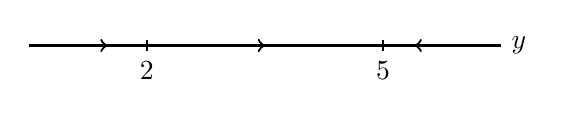
\begin{tikzpicture}[thick]
          \foreach \X in {2, 5} {
            \draw (\X, 2pt) -- (\X, -2pt) node [below] {\(\X\)};
          }
          \foreach \X in {1.5, 3.5} {
            \draw [->] (\X - 0.1, 0) -- (\X, 0);
          }
          \foreach \X in {5.5} {
            \draw [<-] (\X - 0.1, 0) -- (\X, 0);
          }
          \draw (0.5, 0) -- (6.5, 0) node [right] {\(y\)};
        \end{tikzpicture}
      \end{figure}

      The diagram makes it clear that \(y = 2\) is semi-stable and \(y = 5\) is stable.

    \end{solution}

    \pagebreak

    % Problem 7
    \item (3 points) Consider the system
    \begin{equation*}
      \vec{x}' = A \vec{x}, \quad A =
      \begin{pmatrix*}[c]
        -3 & -4 \\
        1 & -1
      \end{pmatrix*}, \quad \vec{x} =
      \begin{pmatrix*}[c]
        x(t) \\
        y(t)
      \end{pmatrix*}
    \end{equation*}
    The eigenvalues of \(A\) are \(\lambda = -2 \pm i \sqrt{3}\).
    Sketch the phase portrait of the system.
    Please indicate the direction of motion on your solution curves, and do not forget to label your axes.

    \begin{solution}
      The complex eigenvalues indicate that the phase portrait is a spiral.
      Since the real part of the eigenvalue is \(-2 < 0\), the spiral points toward the origin as \(t\) increases.

      \begin{figure}[h]
        \centering
        \def\svgwidth{0.9\columnwidth}
        \import{media/}{phasePortrait7.pdf_tex}
      \end{figure}
    \end{solution}

    \pagebreak

    % Problem 8
    \item (5 points) Solve the following initial value problem.
    Solve for \(y\) in terms of \(t\) and leave your answer in terms of a definite integral.
    Show your work.
    \begin{equation*}
      y' + 2ty = 3, \quad t \geq 0, \quad y(0) = 10
    \end{equation*}

    \begin{solution}
      The differential equation is first order linear. The integrating factor is
      \begin{equation*}
        \mu(t) = \exp \left( \int 2t \; dt \right) = e^{t^{2}}
      \end{equation*}
      Multiplying both sides by \(\mu(t)\) yields
      \begin{align*}
        y' e^{t^{2}} + 2ty e^{t^{2}} &= 3e^{t^{2}} \\
        \frac{d}{dt} (y e^{t^{2}}) &= 3e^{t^{2}}
      \end{align*}
      We can integrate both sides to obtain
      \begin{equation*}
        y e^{t^{2}} = \int 3e^{t^{2}} \; dt + C
      \end{equation*}
      I don't know of a pleasant closed form solution to the integral so I'll leave it in that form.
      We can use the initial condition \(y(0) = 10\) to solve for the constant.
      Note that we rewrite the integral with limits to reflect the antiderivative and domain over which \(t\) is defined.
      \begin{gather*}
        10 = \int_{0}^{0} 3e^{x^{2}} \; dx + C \\
        C = 10
      \end{gather*}
      Thus, we can solve for \(y\) and find
      \begin{equation*}
        y(t) = e^{-t^{2}} \left( 3 \int_{0}^{t} e^{x^{2}} \; dx + 10 \right)
      \end{equation*}
    \end{solution}

    \pagebreak

    % Problem 9
    \item (10 points) Consider the IVP.
    \begin{equation*}
      \vec{x}' = A \vec{x} =
      \begin{pmatrix*}[c]
        5 & \frac{1}{2} \\
        -\frac{1}{2} & 4
      \end{pmatrix*} \vec{x}, \quad \vec{x}(0) =
      \begin{pmatrix*}[c]
        2 \\
        1
      \end{pmatrix*}, \quad \vec{x} = \vec{x}(t)
    \end{equation*}

    \begin{enumerate}[label={(\alph*)}]
      \item (2 points) Determine the eigenvalues of \(A\). Show your work.

      \item (5 points) Express the general solution of the IVP in terms of real values functions.

      \item (3 points) Sketch the phase portrait of the system.
      Please include the eigenspaces in your sketch,
      indicate the direction of motion of your solution curves and eigenspaces,
      and do not forget to label your axes.
    \end{enumerate}

    \begin{solution}
      We determine the eigenvalues of \(A\) by finding the roots of the characteristic polynomial.
      The characteristic polynomial is
      \begin{gather*}
        \det(A - \lambda I) = (5 - \lambda) (4 - \lambda) - \left( \frac{1}{2} \right) \left(-\frac{1}{2} \right) =
        \lambda^{2} - 9 \lambda + \frac{81}{4} = 0 \\
        \left(\lambda - \frac{9}{2}\right)^{2} = 0
      \end{gather*}
      Then the eigenvalue is \(\lambda = \frac{9}{2}\) with multiplicity two.
      Consider the system \((A - \lambda I) \vec{x} = 0\).
      \begin{equation*}
        \begin{pmatrix*}[c]
          \frac{1}{2} & \frac{1}{2} \\
          -\frac{1}{2} & -\frac{1}{2}
        \end{pmatrix*}
        \begin{pmatrix*}[c]
          x_{1} \\
          x_{2}
        \end{pmatrix*} =
        \begin{pmatrix*}[c]
          0 \\
          0
        \end{pmatrix*}
      \end{equation*}
      The first row yields the equation
      \begin{equation*}
        \frac{x_{1}}{2} + \frac{x_{2}}{2} = 0
      \end{equation*}
      If \(x_{1} = 2\), then \(x_{2} = -2\). Then the eigenvector is
      \begin{equation*}
        \vec{v}_{1} =
        \begin{pmatrix*}[c]
          2 \\
          -2
        \end{pmatrix*}
      \end{equation*}
      A second eigenvector associated with \(\lambda\) satisfies the equation \((A - \lambda I) \vec{x} = \vec{v}_{1}\), or
      \begin{equation*}
        \begin{pmatrix*}[c]
          \frac{1}{2} & \frac{1}{2} \\
          -\frac{1}{2} & -\frac{1}{2}
        \end{pmatrix*}
        \begin{pmatrix*}[c]
          x_{1} \\
          x_{2}
        \end{pmatrix*} =
        \begin{pmatrix*}[c]
          2 \\
          -2
        \end{pmatrix*}
      \end{equation*}
      The first row yields
      \begin{equation*}
        \frac{x_{1}}{2} + \frac{x_{2}}{2} = 2
      \end{equation*}
      If \(x_{1} = 2\), then \(x_{2} = 2\) so the second eigenvector is
      \begin{equation*}
        \vec{v}_{2} =
        \begin{pmatrix*}[c]
          2 \\
          2
        \end{pmatrix*}
      \end{equation*}
      Then the general solution is
      \begin{equation*}
        \vec{x} = c_{1} e^{\frac{9t}{2}} \vec{v}_{1} + c_{2} e^{\frac{9t}{2}} (\vec{v}_{2} + t \vec{v}_{1})
      \end{equation*}
      Using the inital value yields the system
      \begin{align*}
        2 &= 2 c_{1} + 2 c_{2} \\
        1 &= -2 c_{1} + 2 c_{2}
      \end{align*}
      which has the solution \(c_{1} = 1/4\) and \(c_{2} = 3/4\).
      Thus, the solution to the IVP is
      \begin{equation*}
        \vec{x} = \frac{1}{4} e^{\frac{9t}{2}}
        \begin{pmatrix*}[c]
          2 \\
          -2
        \end{pmatrix*} + \frac{3}{4} e^{\frac{9t}{2}}
        \begin{pmatrix*}[c]
          2 + 2t \\
          2 - 2t
        \end{pmatrix*}
      \end{equation*}
      The phase portrait has one eigenvector, and the solution curves should point outward.
      \begin{figure}[h]
        \centering
        \def\svgwidth{0.9\columnwidth}
        \import{media/}{phasePortrait9.pdf_tex}
      \end{figure}

      The red line denotes the eigenvector and the blue curve is the particular solution to the IVP.
    \end{solution}

    \pagebreak

    % Problem 10
    \item (10 points) Consider the initial value problem.
    \begin{equation*}
      \vec{x}' = A \vec{x}, \quad A =
      \begin{pmatrix*}[c]
        5 & -1 & 2 \\
        2 &  2 & 2 \\
        2 & -1 & 5
      \end{pmatrix*}, \quad \vec{x}(0) =
      \begin{pmatrix*}[c]
        2 \\
        5 \\
        5
      \end{pmatrix*}, \quad \vec{x} = \vec{x}(t)
    \end{equation*}

    \begin{enumerate}[label={(\alph*)}]
      \item Determine the eigenvectors of \(A\) and use them to write down the general solution to the system of differential equations.
      You may use that the eigenvalues of \(A\) are \(\lambda_{1} = 6\) and \(\lambda_{2} = 3\), and one of the eigenvalues has a multiplicity of two.
      \textit{Show your work when computing the eigenvectors:
      it is ok to check your work with software, but you should show that you can compute eigenvectors by hand.}

      \item Use your result from the previous part to solve the IVP.
    \end{enumerate}

    \begin{solution}
      To find the eigenvectors, we first consider the equation \((A - \lambda_{1} I) \vec{x} = 0\).
      Writing the augmented matrix, we can row reduce.
      \begin{align*}
        \begin{pmatrix}[ccc|c]
          -1 & -1 & 2 & 0\\
          2 & -4 & 2 & 0\\
          2 & -1 & -1 & 0
        \end{pmatrix}
        \Longrightarrow
        \begin{pmatrix}[ccc|c]
        1 & 1 & -2 & 0\\
        0 & -6 & 6 & 0\\
        0 & -3 & 3 & 0
      \end{pmatrix}
      \Longrightarrow
      \begin{pmatrix}[ccc | c]
        1 & 0 & -1 & 0 \\
        0 & 1 & -1 & 0 \\
        0 & 0 & 0 & 0
      \end{pmatrix}
      \end{align*}
      The augmented matrix represents the two equations
      \(x_{1} - x_{3} = 0\) and \(x_{2} - x_{3} = 0\).
      Then we have \(x_{1} = x_{2} = x_{3}\) so letting \(x_{1} = 1\) yields the eigenvector
      \begin{equation*}
        \vec{v}_{1} =
        \begin{pmatrix}
          1 \\
          1 \\
          1
        \end{pmatrix}
      \end{equation*}
      Now consider the equation \((A - \lambda_{2} I) \vec{x} = 0\), which creates the augmented matrix
      \begin{equation*}
        \begin{pmatrix}[ccc|c]
          2 & -1 & 2 & 0 \\
          2 & -1 & 2 & 0 \\
          2 & -1 & 2 & 0
        \end{pmatrix}
        \Longrightarrow
        \begin{pmatrix}[ccc|c]
          2 & -1 & 2 & 0 \\
          0 & 0 & 0 & 0 \\
          0 & 0 & 0 & 0
        \end{pmatrix}
      \end{equation*}
      The top row yields the equation \(2x_{1} - x_{2} + 2x_{3} = 0\).
      Letting \(x_{1} = 1\), we can see that setting \(x_{2} = 2\) and \(x_{3} = 0\) yields the eigenvector
      \begin{equation*}
        \vec{v}_{2} =
        \begin{pmatrix}
          1 \\
          2 \\
          0
        \end{pmatrix}
      \end{equation*}
      A second eigenvector is obtained by setting \(x_{2} = 0\) and \(x_{3} = -1\), yielding
      \begin{equation*}
        \vec{v}_{3} =
        \begin{pmatrix}
          1 \\
          0 \\
          -1
        \end{pmatrix}
      \end{equation*}
      Then the general solution to the system of differential equations has the form
      \begin{equation*}
        \vec{x} = c_{1} e^{6t}
        \begin{pmatrix}
          1 \\
          1 \\
          1
        \end{pmatrix} +
        c_{2} e^{3t}
        \begin{pmatrix}
          1 \\
          2 \\
          0
        \end{pmatrix} +
        c_{3} e^{3t}
        \begin{pmatrix}
          1 \\
          0 \\
          -1
        \end{pmatrix}
      \end{equation*}
      Using the initial condition yields the following system, which I represent with an augmented matrix.
      \begin{equation*}
        \begin{pmatrix}[ccc|c]
          1 & 1 & 1 & 2 \\
          1 & 2 & 0 & 5 \\
          1 & 0 & -1 & 5
        \end{pmatrix}
        \Longrightarrow
        \begin{pmatrix}[ccc|c]
          1 & 1 & 1 & 2 \\
          0 & 1 & -1 & 3 \\
          0 & 0 & 1 & -2
        \end{pmatrix}
      \end{equation*}
      which yields the constants \(c_{1} = 3, c_{2} = 1, c_{3} = -2\).
      Thus, the particular solution to the IVP is
      \begin{equation*}
        \vec{x} = 3 e^{6t}
        \begin{pmatrix}
          1 \\
          1 \\
          1
        \end{pmatrix} +
        e^{3t}
        \begin{pmatrix}
          1 \\
          2 \\
          0
        \end{pmatrix} -
        2 e^{3t}
        \begin{pmatrix}
          1 \\
          0 \\
          -1
        \end{pmatrix}
      \end{equation*}
    \end{solution}

  \end{enumerate}
\end{document}
